\chapter{iOS Application}

\section{How to install GetALift (GEA) on your iPhone}

\subsection{Xcode}

To work on the GAL project, you have to use Xcode. Xcode downloads directly on the App Store.
\\\\
To open the project on Xcode, launch Xcode and click on \textit{File/Open} and select in the  \textit{getalift-ios} folder the \textit{GALDev.xcworkspace} and click on \textit{Open}

\subsection{GALDev.xcodeprojet}

\begin{figure}[h!]
\begin{center}
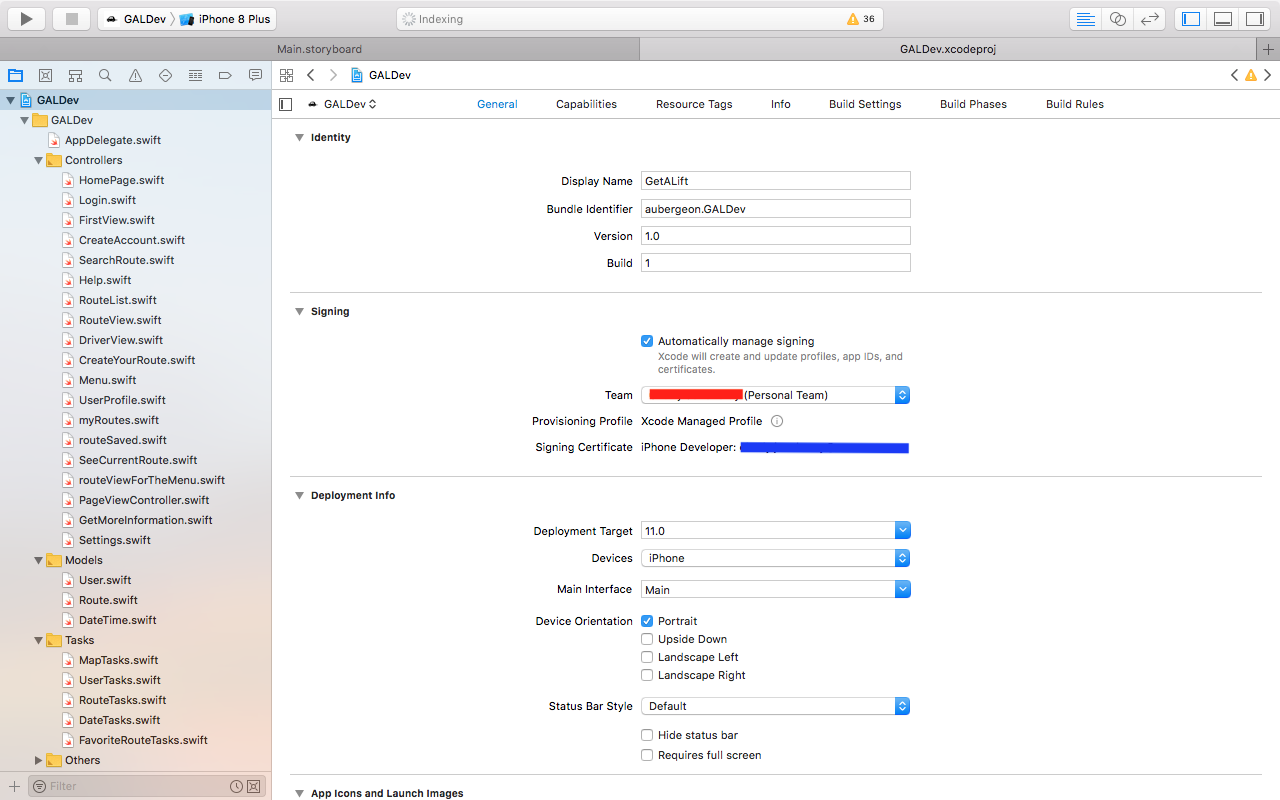
\includegraphics[scale = 0.25]{diagrams/Xcode-General.png} 
\end{center}
\caption{GALDev - General}
\end{figure}
When you open it for the first time you should have errors concerning the \textit{Bundle Identifier}. Take care that it is \textit{yourname.nameoftheproject}.
\\\\
To install the GEA application on your personnal iPhone, you should create a developper account. To create a developper account, go in \textit{Xcode Preferences} and then in \textit{Acount}
\\\\
Click on the "+" and create a new account (cf. figure 5.2). 
\begin{figure}[h!]
\begin{center}
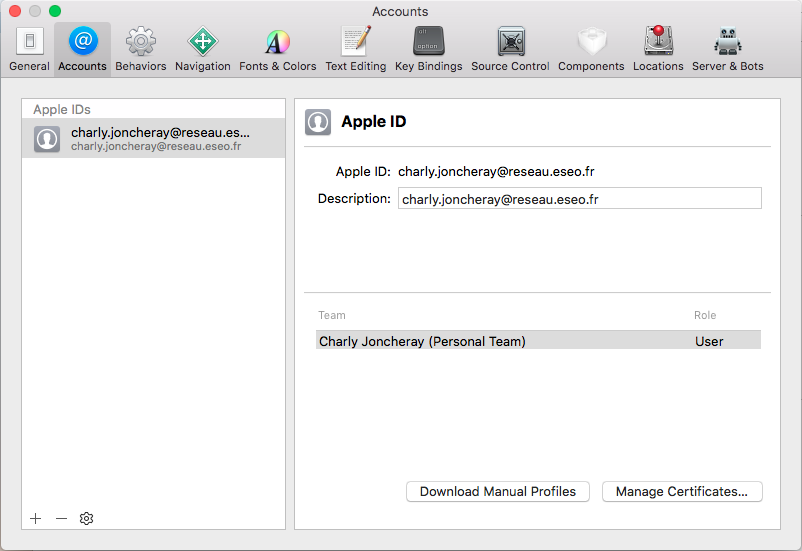
\includegraphics[scale = 0.5]{diagrams/createAnAccount.png} 
\end{center}
\caption{Xcode - Account}
\end{figure}
\\\\
Then, in the \textit{General} page of your project (cf. figure 5.1), select your account as being your \textit{Team} (red box).
\\\\
In the blue box, you should see your email adress.
\\\\
You should have an error concerning the \textit{NotificationBannerSwift}. It because of CocoaPods.

\subsection{CocoaPods}

CocoaPods is a dependency manager for Swift and Objective-C Cocoa projects. It has over 50 thousand libraries. It is used in the GAL application and it is necessary to install it is necessary to install it on your Mac.

\subsubsection{How to install CocoaPods on your Mac}

To install CocoaPods, you have to use the Terminal on your Mac. Open the Terminal.
\\\\
In the folder that contains the project : \textit{/getalift/getalift-ios/} make sure there is the file : \textit{Podfile}
\\\\
If it is not the case, in the Terminal, in the folder containing the xcodeproject file for your project, run the command:
\\\\
\begin{DDbox}{\linewidth}
\begin{verbatim}
pod init
\end{verbatim}
\end{DDbox}
\\\\
This will create a new text file named Podfile (no extension), with the following content:
\\\\
\begin{DDbox}{\linewidth}
\begin{verbatim}
# Uncomment this line to define a global platform for your project
# platform :ios, "7.0"

target 'GALDev' do

end
\end{verbatim}
\end{DDbox}
\\\\
You can delete the first 2 lines of comments. Replace this code by :
\\\\
\begin{DDbox}{\linewidth}
\begin{verbatim}
use_frameworks! #Because we use Swift in the project
target ‘GALDev’ do 
pod 'NotificationBannerSwift'
pod ‘GoogleMaps’
end
\end{verbatim}
\end{DDbox}
\\\\
Then, run the following command line in the Terminal in the folder where the \textit{Podfile} file is located :
\\\\
\begin{DDbox}{\linewidth}
\begin{verbatim}
pod install
\end{verbatim}
\end{DDbox}
\clearpage
\section{GetALift iOS Application}
\begin{figure}[h!]
\begin{center}
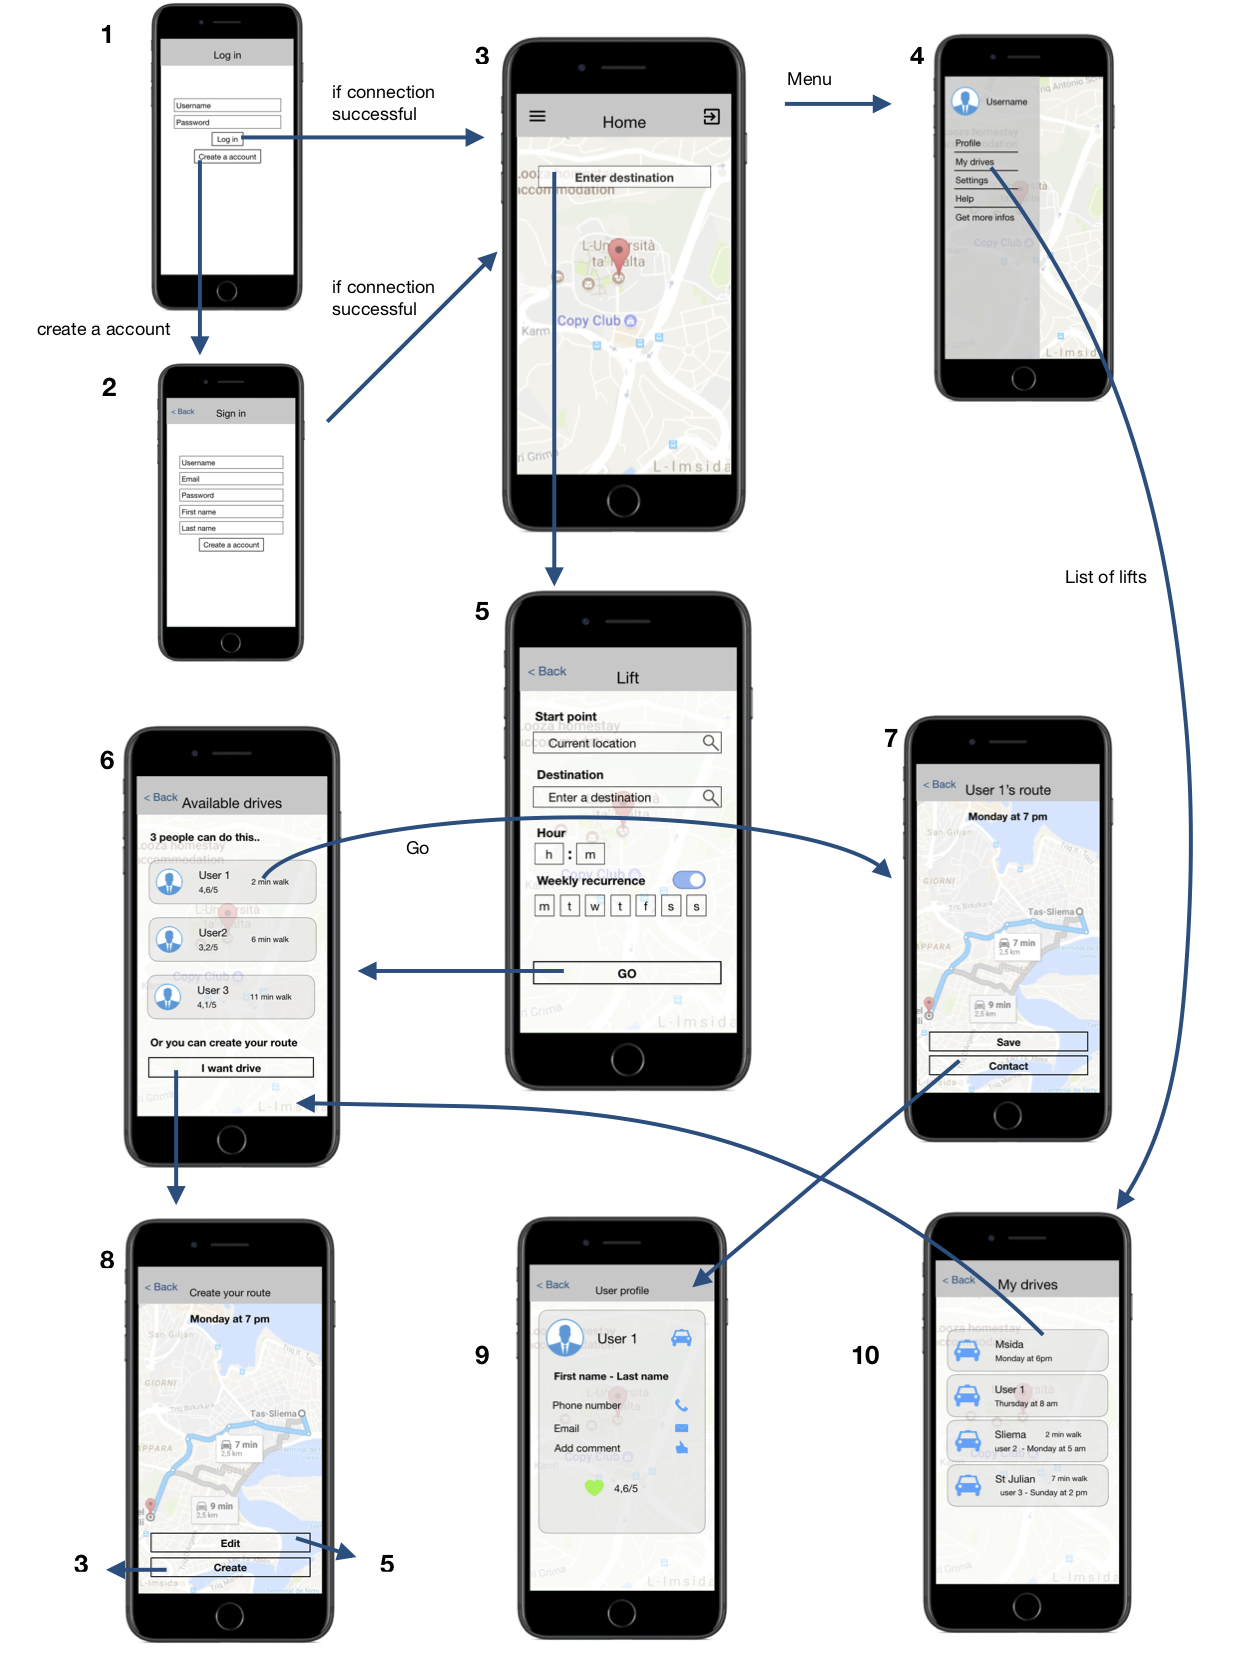
\includegraphics[scale = 0.35]{diagrams/iOSApplication.png} 
\end{center}
\caption{GALDev iOS Application}
\end{figure}

Don't forget to open "GalDev.xcworkspace" in Xcode and not GALDev.xcodeproject otherwise you will have errors.

\subsection{App preview}

\subsubsection{Application homepage}
This is the home page of the app, the one that first appears when the user opens the app. He can access the authentication and account creation page by clicking on the buttons or by making a continuous gesture from left to right on the screen.

\begin{figure}[h!]
\begin{center}
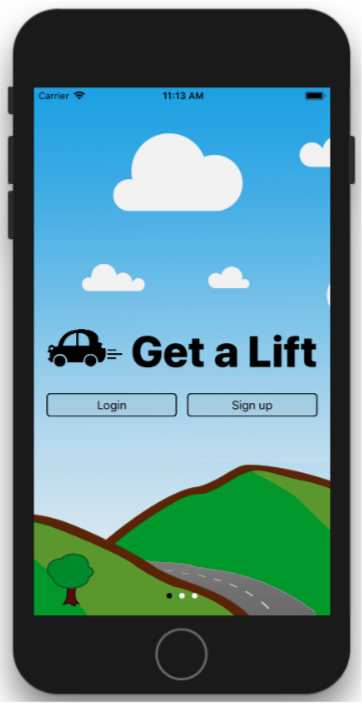
\includegraphics[scale = 0.3]{diagrams/ApplicationHomepage.png} 
\end{center}
\caption{Application homepage}
\end{figure}

\subsubsection{Authentification page}

This page allows the authentication of the user.
\begin{figure}[h!]
\begin{center}
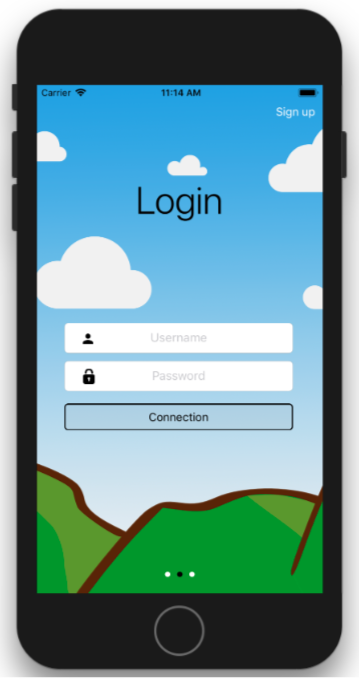
\includegraphics[scale = 0.3]{diagrams/AuthentificationPage.png} 
\end{center}
\caption{Authentification Page}
\end{figure}
When the "Connection" button is pressed, the system checks that all the fields are filled in, otherwise it returns an error message in the form of a notification of this type:
\begin{figure}[h!]
\begin{center}

\includegraphics[scale = 0.3]{diagrams/AuthentificationPageFailed.png} 
\end{center}
\end{figure}
\\\\
Then the system sends the collected information to the database which verifies the authentication.

\subsubsection{Account creation page}

This page allows the creation of an user account.
\\\\
\begin{figure}[h!]
\begin{center}
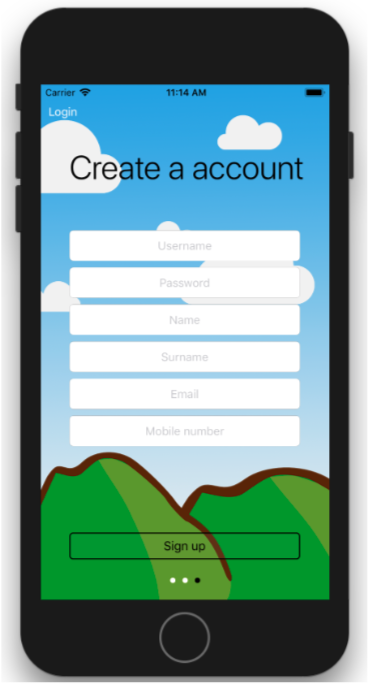
\includegraphics[scale = 0.3]{diagrams/AccountCreationPage.png} 
\end{center}
\caption{Creation Account Page}
\end{figure}
\\\\
When the "Sign up" button is pressed, the system checks that all the fields are filled in, otherwise it returns an error message in the form of a notification.
\\\\
Then the system sends the collected information to the database that creates an account in the database.

\subsubsection{Main page}

Once authenticated, the user arrives on this page, which is the main page of the application. It provides access to the menu and search interface of a route. It also presents a map showing the current position of the user, after authorization of the user.
\\\\
At the top left, there is the button to access the menu and the right is the button to access the search interface of a trip. The button at the bottom right makes it possible to refocus the map on the position of the user.
\\\\
If the user is the driver for routes where the are passengers, alert message will be displayed when he connect. He had to confirm if the passenger was in his car or not. If he click on "Yes", the passenger could see the route in his "MyRides" tab. If he click on "No", the passenger is deleted in the database of the Passenger tab. 

\begin{figure}[h!]
\begin{center}
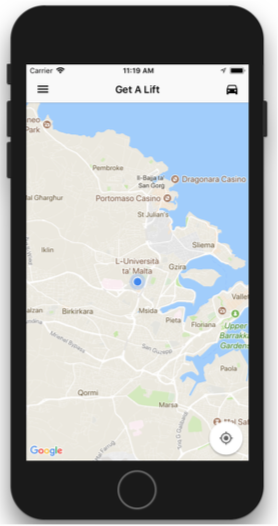
\includegraphics[scale = 0.3]{diagrams/MainPage.png} 
\end{center}
\caption{Main Page}
\end{figure}
\\\\

\subsubsection{Menu}

We can access to different functionality from the menu :
\begin{figure}[h!]
\begin{center}
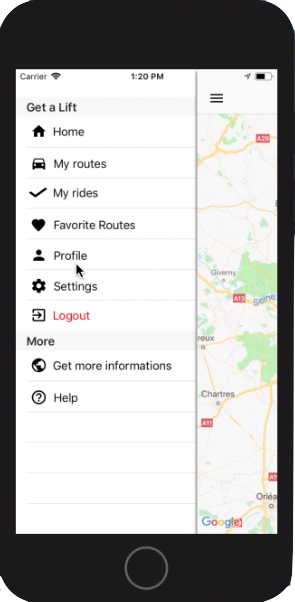
\includegraphics[scale = 0.3]{diagrams/Menu.png} 
\end{center}
\caption{Menu}
\end{figure}

We can :
\begin{itemize}
\item go to the main page
\item see information about his profile
\item get more information about the app
\item access a tutorial to discover how the application works
\item access the application settings
\item Sign out.
\item see the section "My routes" which is the list of the routes that the authenticated user has created as a driver
\item see the section "Favorite Routes" which is the list of trips that the user has saved as a passenger.
\end{itemize}

To access the route search interface, click on the button:
\begin{figure}[h!]
\begin{center}

\includegraphics[scale = 0.3]{diagrams/SearchButton.png} 
\end{center}
\end{figure}

\subsubsection{Search interface of a route}

This interface groups together the search and the creation of a trip in order to highlight carpooling. Indeed, if a user wants to create a route as a driver he will in any case access the list of available routes according to his criteria. This will show this user that other people are making the same trip as him and that he is not obliged to create another trip. This makes it possible to promote carpooling and to simplify the use of the application.

\begin{figure}[h!]
\begin{center}
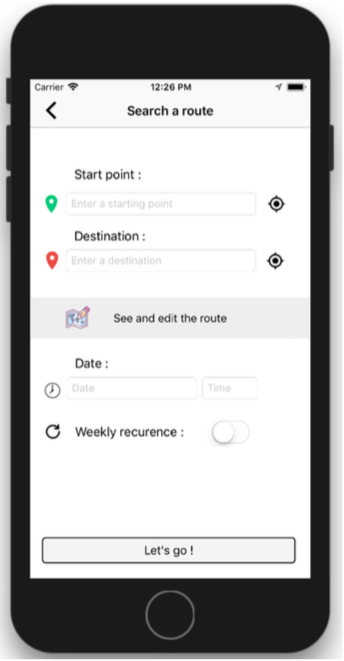
\includegraphics[scale = 0.3]{diagrams/SearchInterfaceRoute.png} 
\end{center}
\caption{Search interface of a route}
\end{figure}

Here we specify its point of departure and its point of arrival. When you click on the text entry field a drop-down menu is displayed to make suggestions to the user. He can also click on the locate button to display the current position of the user in the text entry field.
\\\\
Once this information is entered, the user can display and fine-tune his journey using a map. By clicking on the "See and edit the route" button.
\\\\

\subsubsection{Preview of the desired route}

On this map you can directly edit the points on the map "by hand". The user can zoom, move the map to draw the path that suits him. Whenever the position of a point is changed, the path between the two points is updated. Once the route has been modified, the user can return to the search page of a trip and the input fields will be immediately modified to display the coordinates of the points he has previously modified on the map.

\begin{figure}[h!]
\begin{center}
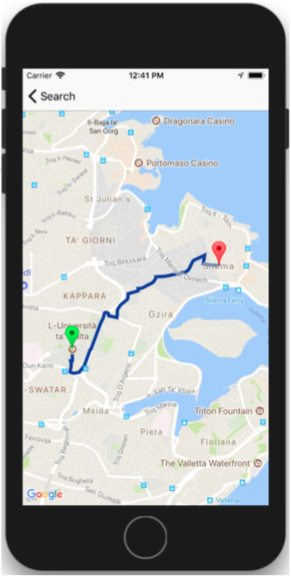
\includegraphics[scale = 0.3]{diagrams/PreviewRoute.png} 
\end{center}
\caption{Preview of the desired route}
\end{figure}

The user can now enter the date and time of his trip in the search interface of a route. He can also notify if his trip will be done every week or not. The purpose of this application is to connect the users of the daily road.
\\\\
Once all fields are completed, he can click on the "Let's go" button to display the corresponding results.
\\\\

\subsubsection{List of available routes}

\begin{figure}[h!]
\begin{center}
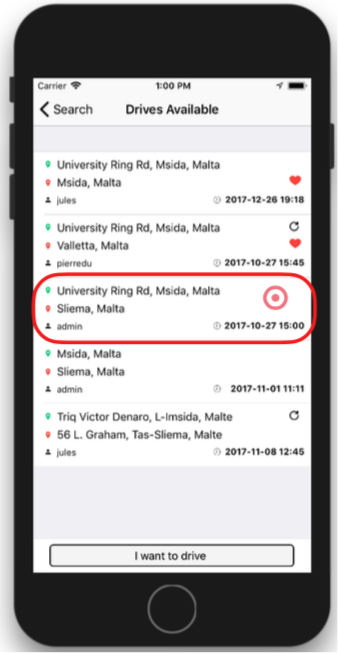
\includegraphics[scale = 0.3]{diagrams/ListAvailableRoutes.png} 
\end{center}
\caption{List of available route}
\end{figure}

We can observe several routes available with information about them (date, time, driver, recurrence). The red heart indicates that it is a road registered as a favorite road.
\\\\
The button offers the possibility to create its own route.
\\\\
If we click on the route, the next page is displayed with the route projection on a map and the different route information.
\\\\

\subsubsection{Overview of a route}

\begin{figure}[h!]
\begin{center}
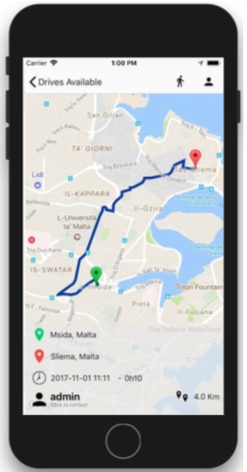
\includegraphics[scale = 0.3]{diagrams/OverviewRoute.png} 
\end{center}
\caption{Overview of a route}
\end{figure}

In this view we find all the information on the trip. We can see the road on a map and if we click on the button representing a man who walks, we will have the way to walk between our starting point and that of the path that will be displayed, and the same for the point of departure. Just press this button again to remove the path to walk.
\\\\
The user can also access the driver's information to contact him or save the trip by clicking on his or her pseudonym or by clicking on the small contact icon at the top right of the screen.
\\\\

\subsubsection{Overview of a driver}

\begin{figure}[h!]
\begin{center}
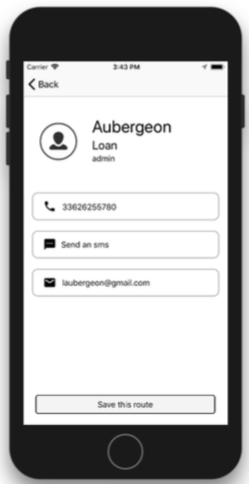
\includegraphics[scale = 0.3]{diagrams/OverviewDriver.png} 
\end{center}
\caption{Overview of a driver}
\end{figure}

The user can call him driver, send him an SMS or an email directly from the application by pressing the dedicated buttons. It can also save this trip to its preferred route list to keep it.


\subsubsection{Interface to create a route}

\begin{figure}[h!]
\begin{center}
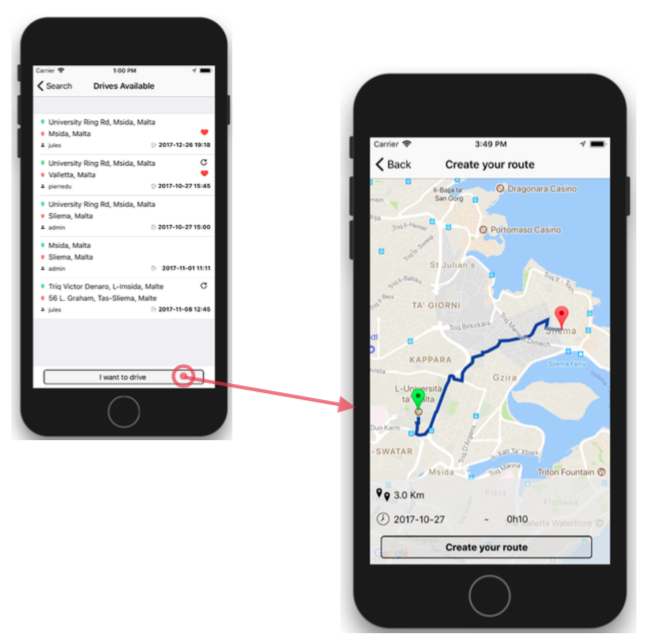
\includegraphics[scale = 0.3]{diagrams/CreateRoute.png} 
\end{center}
\caption{Interface to create a route}
\end{figure}
In the case where the user does not find corresponding paths to his trip, he can create a trip by returning to the list of available trips and clicking on the button "I want to drive".
\\\\
We get a summary page of the route that we want to create, if we want to change this it will be enough to go back and change what we want in the search interface / creation. The user presses the "Create your route" button to finalize the creation, a confirmation alert will be displayed on the screen and the user will be redirected to the main page of the application.
\\\\

\subsubsection{List of created routes}

\begin{figure}[h!]
\begin{center}
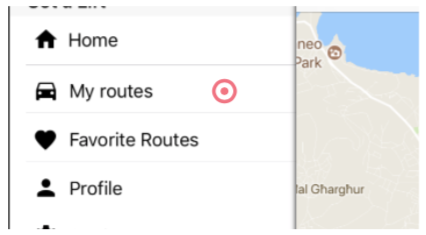
\includegraphics[scale = 0.3]{diagrams/ListCreatedRoute.png} 
\end{center}
\caption{List of created route}
\end{figure}

The user to find this trip in the list of routes he has created, available in the application menu. From this list, the user can see in more detail the routes he has created and delete them.
\\\\
Likewise with the list of his favorite journeys.






















